\documentclass[../report.tex]{subfiles}

\begin{document}
\graphicspath{{img/}{../img/}}

\section*{Target-Projekt}
I denne rapport vil vi studere et projekt vi selv laver i ITU kurset "Second Year Project: Software Development in Large Teams with International Collaboration". I target-projektet skal vi samarbejde med en gruppe studerende fra Singapore Management University om at udvikle et system til at uploade og downloade mediefiler. Systemet kommer til at have to individuelle front-ends, men et delt backend. Derudover skal vi dokumentere designet af systemet og vores samarbejde med de singaporeanske studerende.

\section*{Problemformulering}
I denne rapport vil vi svare p� f�lgende sp�rgsm�l i forhold til vores target-projekt.
\\ \\	
\textbf{Hvordan kan man planl�gge og udf�re et eksamensprojekt s� som vores target-projekt p� en god m�de?}
\begin{enumerate}
	\item	Hvordan kan man estimere hvor lang tid hver subtask i target-projektet tager?
	\item 	Hvordan kan man afveje hvor lang tid man har estimeret projektet tager i forhold til hvor lang tid man har til r�dighed med henblik p� at opn� det bedst mulige resultat?
	\item 	Hvordan kan man v�lge en passende procesmodel i target-projektet?
	%\item 	How can you manage resources and keep the target project on track?
	\item 	Hvilke dele af projektet kunne v�re blevet gjort bedre for at opn� et bedre resultat?
\end{enumerate}

\section*{Metode}
%To answer the problem statement we will look at the tools used in the target project. Additionally we will apply other tools to the target project and evaluate the different results. Using these tools include doing calculations and creating diagrams.

For at svare p� problemformuleringen vil vi kigge p� forskellige metoder til at estimere, planl�gge og udf�re aktiviteter i vores target-projekt. I target-projektet vil vi anvende Delphi-metoden til at estimere vores aktiviteter med, en simplificerert version af SCRUM (SCRUM-but) som procesmodel og et Gantt kort til planl�gning af vores aktiviteter. Derudover vil vi sidel�bende afpr�ve alternative metoder vi kan sammenligne med de metoder vi faktisk bruger i projektet. Dette vil inkludere Function Points til estimering af aktiviteter, vandfaldsmodellen og spiralmodellen som procesmodeller og The Precendence Network til at planl�gge aktiviteter. 

%Forskellige estimeringsmetoder: FP, Delphi
%Forskellige processmodeller: Vandfald, SCRUM, spiral
%Forskellige aktivitetsplanl?gningsmetoder: precedence network (critical path), gantt


\newpage
\newgeometry{left=7cm,bottom=1.5cm}
\begin{landscape}

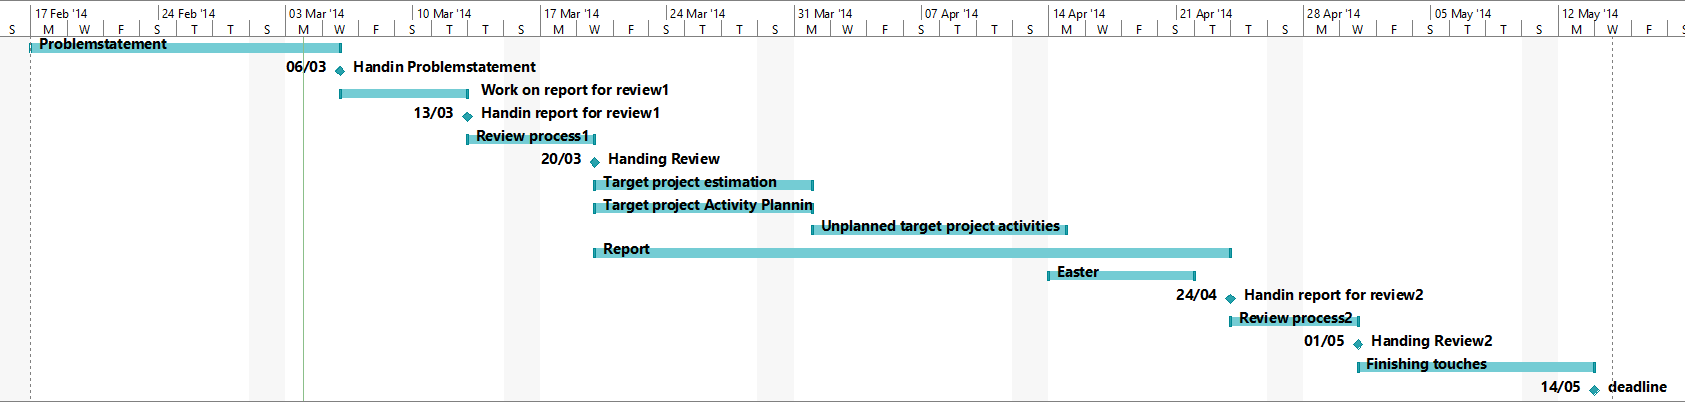
\includegraphics[ scale=0.57]{timeschedule.png}


\end{landscape}


\restoregeometry

\end{document}
